\chapter{Konzeption}

In diesem Kapitel wird die Konzeption des Gesamtsystems beschrieben. Es wird die Nutzungskontextanalyse beschrieben, welches als Grundlage und Vorbereitung für die anschließende Anforderungsanalyse diente. Die Anforderungsanalyse in welcher, im Rahmen eines Kreativ Workshops, Anwendungsfälle für das zu konzipierende System erarbeitet wurden, wird erläutert. Abschließend wird einEntwurf der Anwendung beschrieben.

\section{Nutzungskontextanalyse}

% Aktuelle Problemlösungstrategien? Bewertungen auf Online Portalen, Blogs, Interessengruppen, Reklamationen, Technischer Support
Aktuelle Lösungen für die Abgabe von Rückmeldungen zur Gestaltung von Produkten erfolgt oft ohne den Einsatz von Augmented Reality. Diese erfolgen 
oft als Bewertungen in Online Einkaufsportalen, Blog Beiträgen, durch den Austausch in Interessengruppen oder über direkten Kontakt zum Hersteller, die 
meist über die Kontaktaufnahme zum technischen Support erfolgt.

Bei Bewertungen in Onlineportalen, in Blog Beiträgen oder auch bei direktem Kontakt zum Hersteller (z.Bsp. durch E-Mail), haben Kunden die Möglichkeit 
ihre Gestaltungsidee schriftlich zu beschreiben und mit Bildern oder Videos zu ergänzen. Bei solchen Beschreibungen kommt es jedoch manchmal vor dass 
nicht immer klar hervorgeht zu welcher Stelle oder zu welchem Teil am Produkt sich die Beschreibung bezieht. Die Umgebung als Kontext in welchem das Produkt 
verwendet wird geht aus solchen Beschreibungen nicht immer hervor. Zudem ist nicht ohne Aufwand möglich direkt zu erkennen an welchen Stellen eines Produktes 
welche Rückmeldungen häufen. \footnote{Z.Bsp.: Angenommen es gibt zum Produkt sehr viele unterschiedliche Rückmeldungen. Mit direktem Blick zu erkennen dass 
die meisten Rückmeldungen bei einem Produkt, beispielsweise einer Kaffeetasse auf die untere Kante am Griff beziehen.} 

Bei Interessengruppen in welchen Nutzer von bestimmten Produkten sich an einem Ort treffen um Erfahrungen auszutauschen wie z.Bsp. bei Hausaltprodukten, Modellflugzeugen, VR Brillen etc., 
haben die Nutzer die Möglichkeit ihre Ideen genauer, mit Bezugnahme auf stellen am Produkt und dem Kontext ihrer Umgebung zu beschreiben. Das Problem bei dieser Art 
der Rückmeldungen ist jedoch dessen eingrenzte Reichweite. Zudem werden Inhalte welche in solchen Treffen diskutiert wurden oft nicht ausreichend dokumentiert.  

Auf Basis der im Kapitel \ref{CapterFundamentals} behandelten Grundlagen und der Nutzungskontextanalyse wurde eine erste Skizze des Gesamtsystems entworfen in welcher, 
Funktionale wie Nicht-Funktionale Anforderungen an das zu konzipierende System skizziert wird (siehe Abbildung \ref{img:sysstem_sketch}).

\begin{figure}[H]
	\centering
	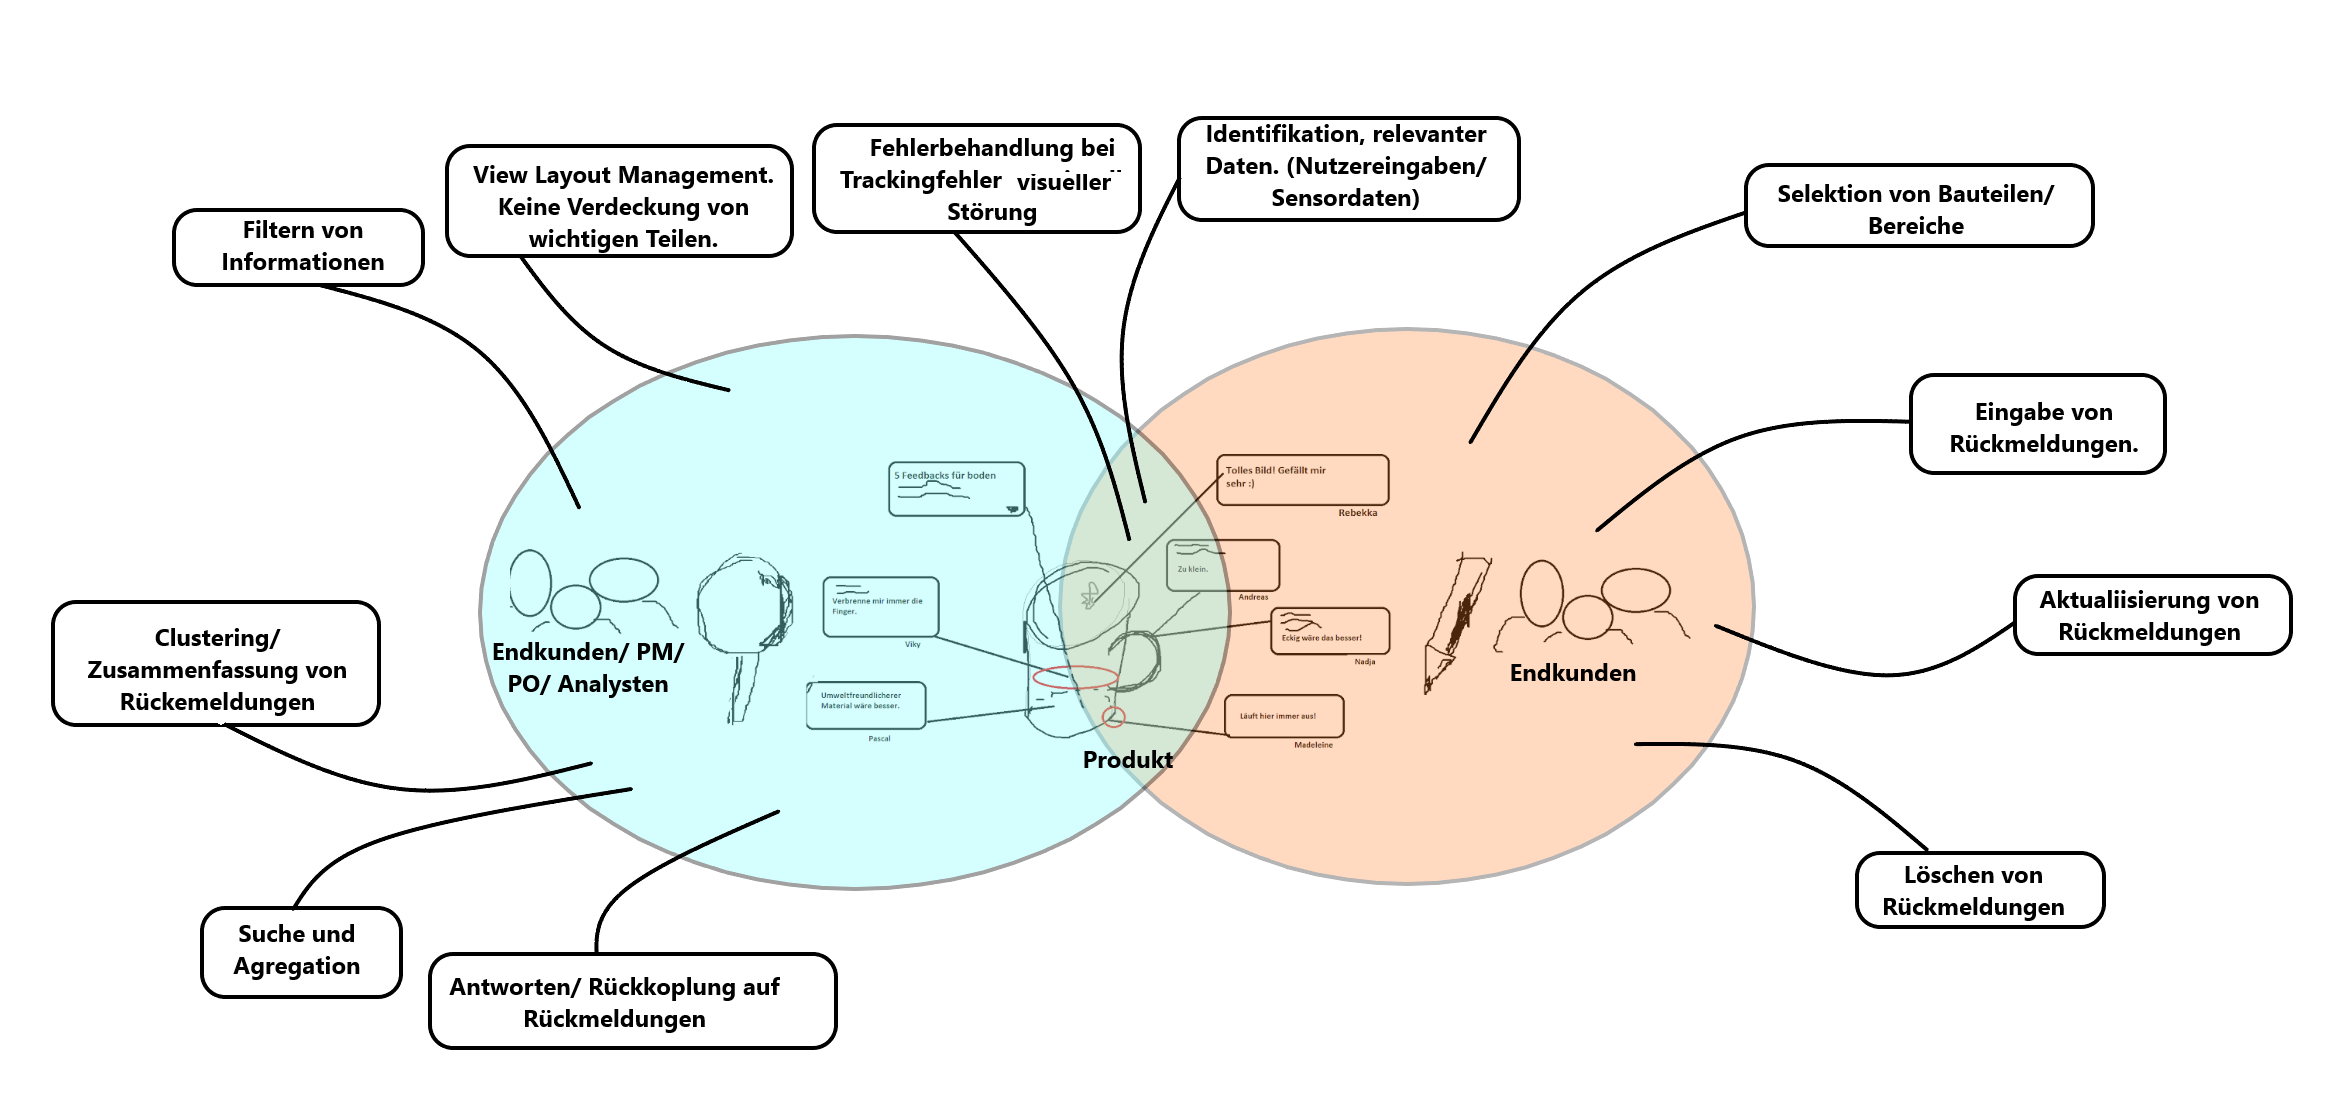
\includegraphics[width=1.0\textwidth]{resources/conception/skizze_gesamtsystem.png}
	\caption{Skizze des Gesamtsystems als erster Entwurf \cite{system sketch}}
	\label{img:sysstem_sketch}
\end{figure}

Dieses Skizze sollte die Projektidee begreifbarer machen und als grobe Orientierung bei der Anforderungsanalyse dienen.

\subsection{Anforderungsanalyse/ Kreativ Workshop}

Die Anforderungsanalyse wurde im Rahmen eines Kreativ Workshops durchgeführt. Ziel des Workshops war es Die Nutzer für das zu konzipierende System zu identifizieren und deren Eigenschaften und Bedürfnisse 
zu analysieren. 

% Vorbereitung
Das Workshop fand am dritten Juli, am Fraunhofer IPK in Berlin statt. Zur Vorbereitung wurde in einem Besprechungsraum, einzelne Stationen für die am Workshop durchzuführenden Aktivitäten vorbereitet. 
Zunächst wurden die Teilnehmer begrüßt   
  

%Durchführung %Aufbau / Einleitung / Affinitätsdiagram / Personas / Szenarien

% User Stories


\subsubsection{Personas}

\subsubsection{Szenarien}

\subsubsection{Anforderungen}

\textbf{User Stories}

\textbf{Funktionale Anforderungen}

\textbf{Nicht funktionale Anforderungen}

\textbf{Qualitätskriterien und Priorisierung der Anforderungen}

\section{Entwurf}

\subsection{Low-Fidelity-Prototypen}

\subsection{Ergebnis der Prototypen}
(Wizard of Oz Methode)

\subsection{Vorstellung eines Prototypen}
